\documentclass[11pt,a4paper]{article}
\usepackage[margin=2.3cm]{geometry}
\usepackage{booktabs}
\usepackage{graphicx}
\usepackage{amsmath}
\usepackage{microtype}
\usepackage[font=small,labelfont=bf]{caption}
\usepackage[hidelinks]{hyperref}
\setlength{\parskip}{0.4em}
\setlength{\parindent}{0pt}
\renewcommand{\arraystretch}{1.1}

\title{CS623 Assignment 2: CUDA Programming\\[2pt]\large 3D Convolution, 10-D Grid Search, and Counting Bloom Filters}
\author{Dweep Joshipura (Roll No.\ 230395)}
\date{}

\begin{document}
\maketitle

\section{Setup}
Problems 2 and 3 were run on the GPU3 server: NVIDIA A40 (sm\_86, 46\,GB), Intel Xeon Silver 4208 (2.1\,GHz base), CUDA 12.6, driver 590.48.
Problem~1 was run on an NVIDIA RTX 4060 Laptop GPU with an Intel Core i7-14650HX.
All code is built with the provided \texttt{Makefile} (\texttt{make}; \texttt{ARCH=sm\_86} by default, override with \texttt{make ARCH=sm\_80}).
Problem~2 uses \texttt{-{}-fmad=false}, and v3 additionally uses \texttt{-Xcompiler -ffp-contract=off}, so that results match the CPU code bit for bit.

Problem~2 times are wall-clock; Problem~1 and~3 kernel times use CUDA events. Run counts are given with each table; Problem~2 reports medians because the server is shared and a few runs were up to 2$\times$ slower.

\section{Problem 1: 3D convolution}
\textbf{Implementation.}
The basic kernel uses one thread per output element and reads the input and filter directly from global memory.
The optimized kernel uses $8{\times}8{\times}8$ thread blocks that load a $12{\times}12{\times}12$ input tile (with halo) into shared memory, keeps the $5{\times}5{\times}5$ filter in constant memory, and fully unrolls the filter loops.
Out-of-range elements are treated as zero, and both kernels are checked against the single-threaded CPU version.

\textbf{Results.}
Table~\ref{tab:p1} gives means over 10 runs for $N\in\{64,128,256\}$. GPU and CPU outputs matched in all runs.

\begin{table}[h]
\centering\small
\resizebox{\linewidth}{!}{\begin{tabular}{rrrrrrrr}
\toprule
$N$ & CPU & \multicolumn{2}{c}{Basic (ms)} & \multicolumn{2}{c}{Optimized (ms)} & \multicolumn{2}{c}{Speedup} \\
 & (ms) & kernel & end-to-end & kernel & end-to-end & kernel & end-to-end \\
\midrule
64 & 65.4 & 0.517 & 1.97 & 0.052 & 1.46 & 10.0$\times$ & 1.35$\times$ \\
128 & 496.1 & 2.111 & 10.75 & 0.323 & 8.75 & 6.5$\times$ & 1.23$\times$ \\
256 & 3849.2 & 15.346 & 80.82 & 2.505 & 67.25 & 6.1$\times$ & 1.20$\times$ \\
\bottomrule
\end{tabular}}
\caption{Problem 1: mean times over 10 runs. End-to-end includes host--device copies.}
\label{tab:p1}
\end{table}

The optimized kernel is 6--10$\times$ faster than the basic one, since each input element loaded into shared memory is reused by up to 125 outputs and the filter reads become constant-memory broadcasts.
End-to-end the gain is only 1.2--1.35$\times$, because the PCIe transfers dominate once the kernel is fast (at $N=256$ the optimized kernel is 2.5\,ms of a 67\,ms total).
Compared with the CPU, the optimized GPU path is about 45$\times$ ($N=64$) to 57$\times$ ($N=256$) faster end-to-end.

\section{Problem 2: 10-D grid search}
The search space is $13^{10}\approx1.4\times10^{11}$ points (13 values per dimension), of which 11\,608 satisfy all ten constraints.

\textbf{Implementation.}
\begin{itemize}\setlength\itemsep{0pt}
\item \textbf{v0:} the given serial C code.
\item \textbf{v1 (vanilla port):} one thread per grid point (index decoded in mixed radix), problem data in constant memory, hits appended with \texttt{atomicAdd} to a bounded buffer; the space is processed in chunks of $2^{28}$ points over several launches, and the host writes the file.
\item \textbf{v2 (optimized):} one thread per $(x_1..x_7)$ prefix, which reuses the partial sums while looping over $x_8..x_{10}$; hits are reserved with one warp-aggregated \texttt{atomicAdd}. \emph{Pruning:} all coefficients and grid values are non-negative, so partial sums only grow and a loop stops once a constraint is already violated (disabled automatically if the inputs are not non-negative).
\item \textbf{v3 (Thrust):} \texttt{thrust::copy\_if} over a \texttt{counting\_iterator} with a predicate functor, in chunks of $2^{25}$ indices; hit indices are decoded on the host.
\end{itemize}

\textbf{Results.}
Table~\ref{tab:p2} compares the versions. Timing covers the search, copies back and file writing (not start-up). Every version finds 11\,608 points, and its sorted output is identical to v0's.

\begin{table}[h]
\centering\small
\resizebox{\linewidth}{!}{\begin{tabular}{llrrrrr}
\toprule
Version & Description & Runs & Median (s) & Min--Max (s) & vs.\ v0 & vs.\ v1 \\
\midrule
v0 & Serial CPU (reference) & 1 & 657.388 & -- & 1.0$\times$ & 0.05$\times$ \\
v1 & Vanilla CUDA port & 5 & 29.928 & 29.927--30.155 & 22.0$\times$ & 1.0$\times$ \\
v2 & v2, no pruning & 5 & 5.542 & 5.542--5.543 & 118.6$\times$ & 5.4$\times$ \\
v2 & v2 + pruning (final) & 3 & 0.140 & 0.139--0.140 & 4701.7$\times$ & 214.0$\times$ \\
v3 & Thrust & 5 & 40.235 & 40.112--64.975 & 16.3$\times$ & 0.74$\times$ \\
\bottomrule
\end{tabular}}
\caption{Problem 2: total time on the A40 (v0 on the server CPU). v2 + pruning is the final version (block size 128, 3 runs).}
\label{tab:p2}
\end{table}

v2 is 5.4$\times$ faster than v1 even without pruning (partial-sum reuse, far fewer atomics), and pruning gives a further 40$\times$ (5.54\,s to 0.14\,s) because most of the space is cut off early in the inner loops.
The Thrust version is slower than v1 (0.74$\times$): it re-evaluates every point from scratch and cannot prune, and \texttt{copy\_if} adds extra passes.
The first v3 run (65\,s) was an outlier; the others were about 40\,s.

\textbf{Launch configuration and pruning ablation} (Figure~\ref{fig:p2abl}).
v1 is insensitive to the block size (about 30\,s for 64--1024 threads; the 39\,s median at 128 reflects a noisy run). v2 is also flat from 64 to 512 threads.
With 1024 threads v2 fails to launch: it uses 100 registers per thread, and $1024\times100$ exceeds the 65\,536 registers available to one block. Pruning gives a 36--41$\times$ gain at every block size.

\begin{figure}[h]
\centering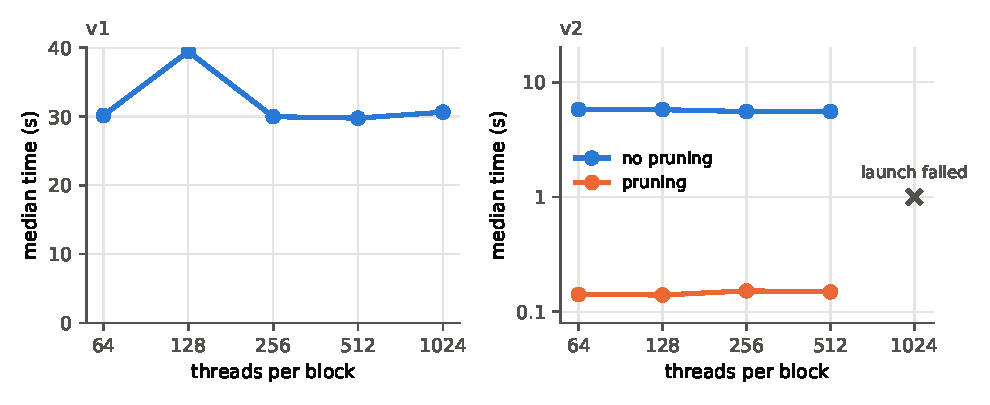
\includegraphics[width=0.85\linewidth]{figures/p2_ablation.pdf}
\caption{Median time versus threads per block (3 runs per point).}
\label{fig:p2abl}
\end{figure}

\section{Problem 3: Counting Bloom filter}
\textbf{Implementation.}
The filter is a raw array of 8-bit counters, packed four per 32-bit word and updated with an \texttt{atomicCAS} loop on the word (CUDA has no 8-bit CAS).
There is one thread per key (grid-stride loop, 256 threads per block), with separate \texttt{insert}, \texttt{delete} and \texttt{search} kernels and $k=3$ hash functions (\texttt{hash1}--\texttt{hash3}).
Duplicates in the insert and delete traces are removed on the host. A delete only decrements if all three counters are non-zero, so deleting an absent key does nothing.
The \emph{blocked} variant adds \texttt{hash4}, which picks a block of 32 counters (32 bytes, one L2 sector); \texttt{hash1}--\texttt{hash3} choose counters inside that block.
\texttt{check\_result()} replays the operations on a \texttt{std::unordered\_set} and counts false negatives (none occurred in any run) and false positives.

\textbf{Trace and metrics.}
The traces have $10^6$ insert keys (950\,000 distinct), $10^6$ search keys (50\% inserted), and 300\,000 delete keys (285\,000 distinct). Unless stated otherwise $N=20\times10^6$ counters. The false-positive rate is false positives divided by all searches; because half of the searches are for absent keys, it cannot exceed 50\%.

\subsection{Performance and false positives}
\begin{table}[h]
\centering\small
\begin{tabular}{lrrr}
\toprule
Kernel & Vanilla (ms) & Blocked (ms) & Blocked / vanilla \\
\midrule
Insert (950\,000 keys) & 1.125 $\pm$ 0.009 & 1.097 $\pm$ 0.034 & 0.98 \\
Search after insert (10$^6$) & 0.231 $\pm$ 0.003 & 0.173 $\pm$ 0.002 & 0.75 \\
Delete (285\,000 keys) & 0.379 $\pm$ 0.002 & 0.347 $\pm$ 0.013 & 0.92 \\
Search after delete (10$^6$) & 0.209 $\pm$ 0.001 & 0.161 $\pm$ 0.003 & 0.77 \\
\bottomrule
\end{tabular}
\caption{Kernel times (mean $\pm$ s.d.\ of 5 runs), $N=20$M.}
\label{tab:p3time}
\end{table}

Blocked search is 25\% faster and delete 8\% faster, while insert is unchanged (Table~\ref{tab:p3time}); insert time is dominated by the \texttt{atomicCAS} loop.

\begin{table}[h]
\centering\small
\begin{tabular}{rrrrr}
\toprule
& \multicolumn{2}{c}{After insert (\%)} & \multicolumn{2}{c}{After delete (\%)} \\
$N$ & Vanilla & Blocked & Vanilla & Blocked \\
\midrule
1M & 41.806 & 40.752 & 41.979 & 40.386 \\
5M & 4.103 & 4.398 & 2.319 & 2.708 \\
10M & 0.773 & 1.024 & 0.396 & 0.613 \\
20M & 0.119 & 0.229 & 0.055 & 0.144 \\
\bottomrule
\end{tabular}
\caption{False-positive rate (\% of all searches) versus filter size $N$.}
\label{tab:p3fp}
\end{table}

The price is a higher false-positive rate (Table~\ref{tab:p3fp}, Figure~\ref{fig:nsweep}): at $N=20$M, blocked gives 0.229\% against 0.119\% after the inserts.
At $N=1$M ($\approx$ one counter per key) both filters are saturated at about 41\%, and the rate falls steeply as $N$ grows.

\begin{figure}[h]
\centering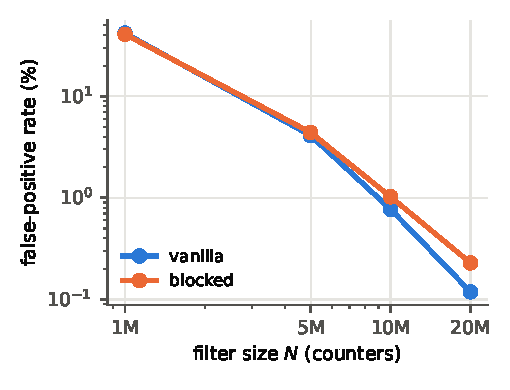
\includegraphics[width=0.5\linewidth]{figures/p3_nsweep.pdf}
\caption{False-positive rate after the inserts versus $N$.}
\label{fig:nsweep}
\end{figure}

\subsection{Block size ablation}
\begin{table}[h]
\centering\small
\begin{tabular}{rrrrr}
\toprule
Block size & Bytes & FP after insert (\%) & Search (ms) & Insert (ms) \\
\midrule
16 counters & 16 & 0.315 & 0.170 & 1.074 \\
32 counters & 32 & 0.229 & 0.175 & 1.040 \\
64 counters & 64 & 0.183 & 0.195 & 1.070 \\
128 counters & 128 & 0.153 & 0.208 & 1.065 \\
256 counters & 256 & 0.134 & 0.223 & 1.080 \\
\midrule
vanilla (no blocks) & -- & 0.119 & 0.231 & 1.125 \\
\bottomrule
\end{tabular}
\caption{Blocked variant, $N=20$M, 3 runs per setting; last row is the vanilla filter.}
\label{tab:blocks}
\end{table}

\begin{figure}[h]
\centering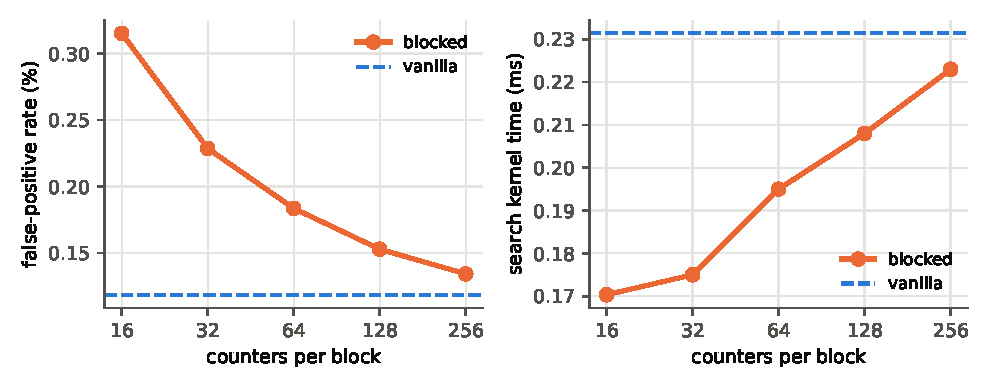
\includegraphics[width=0.85\linewidth]{figures/p3_blocks.pdf}
\caption{Effect of the block size: false positives (left) and search time (right).}
\label{fig:blocks}
\end{figure}

Larger blocks lower the false-positive rate (0.315\% to 0.134\%, approaching vanilla's 0.119\%) but make search slower (0.170\,ms to 0.223\,ms, approaching vanilla's 0.231\,ms).
With 32 counters (32\,B) all three counters of a key lie in a single sector. This is consistent with 32 counters being a good trade-off, and it is the default.

\subsection{Nsight Compute profile}
The first \texttt{insert} and first \texttt{search} kernel launches were profiled for both variants at $N=20$M (\texttt{ncu -{}-set full}); delete was not profiled.

\begin{table}[h]
\centering\small
\resizebox{\linewidth}{!}{\begin{tabular}{lrrrr}
\toprule
 & \multicolumn{2}{c}{Vanilla} & \multicolumn{2}{c}{Blocked} \\
Metric & insert & search & insert & search \\
\midrule
Duration & 1040\,$\mu$s & 219\,$\mu$s & 988\,$\mu$s & 160\,$\mu$s \\
DRAM throughput (\% of peak) & 64.8 & 79.7 & 62.0 & 74.6 \\
Achieved DRAM bandwidth (GB/s) & 451 & 554 & 431 & 519 \\
Arithmetic intensity (int.\ ops/byte) & 0.18 & 0.58 & 0.19 & 0.81 \\
Achieved occupancy (\%) & 85.5 & 91.6 & 83.5 & 81.7 \\
Warp efficiency (\%) & 88.7 & 88.9 & 87.2 & 87.7 \\
L2 hit rate (\%) & 17.4 & 11.9 & 27.6 & 29.6 \\
Long-scoreboard stall (cycles/instr.) & 1311 & 357 & 1342 & 254 \\
\bottomrule
\end{tabular}}
\caption{Nsight Compute metrics. Arithmetic intensity is thread-level integer instructions per DRAM byte (the kernels execute no floating-point instructions). Warp efficiency is the average number of active threads per warp divided by 32.}
\label{tab:ncu}
\end{table}

All four kernels are memory bound: the profiler reports memory throughput (62--80\% of peak DRAM bandwidth) far above compute throughput (1--4\%).
The blocked variant has the better L2 hit rate (28--30\% against 12--17\%) and moves less data from DRAM (search 83\,MB against 122\,MB, insert 426\,MB against 469\,MB), which is consistent with its faster search.

\textbf{Top three bottlenecks reported by the profiler:}
\begin{enumerate}
\item \textbf{Uncoalesced global accesses.} Counter lookups are random, so 85\%/80\% (vanilla insert/search) and 85\%/80\% (blocked) of the transferred sectors are excess; estimated speedup if fixed: 85.12\%/77.97\% (vanilla), 84.98\%/77.24\% (blocked).
\item \textbf{Long-scoreboard stalls.} Warps wait on L1TEX/global loads: 1311.2/356.9 cycles per issued instruction (vanilla insert/search) and 1341.8/254.4 (blocked).
\item \textbf{Poor DRAM/L2 access pattern.} Only 5.1--5.6 of every 32 bytes in a fetched sector are used, and 90.4\%/89.6\% of sectors miss L2 in vanilla versus 71.3\%/72.1\% in blocked.
\end{enumerate}
\vspace{-0.5em}
Atomics were not flagged separately. The generic ``compute pipelines under-utilized'' rule is also reported, but it only restates that the kernels are memory-latency bound.

\end{document}
